\documentclass[12pt]{article}
\usepackage{times}
\usepackage{amsmath,amssymb,amsthm,amsfonts,bm}
\usepackage{bm}
\usepackage{natbib}
% \usepackage[T1]{fontenc}
% \usepackage[utf8]{inputenc} 
\usepackage{enumitem}
\usepackage{hyperref}
\usepackage{lipsum}
\usepackage[ruled]{algorithm2e}
\usepackage{graphicx}
\usepackage{booktabs}
\usepackage{multirow}
\usepackage{indentfirst}
\usepackage{xeCJK}
\setlength{\parindent}{2em}
% \setCJKmainfont{BabelStone Han}
\renewcommand{\refname}{参考文献}
\newcommand{\hl}[1]{{\leavevmode\color{red}{#1}}}

%%%%%%%%%%%%%%%%%%%%%%%%%%%%%%%%%%%%%%%%%%%%%%%%
%% Do not change the following format settings !
%%%%%%%%%%%%%%%%%%%%%%%%%%%%%%%%%%%%%%%%%%%%%%%%
% --- list setting of R code --- %%
\usepackage[svgnames]{xcolor}
\usepackage{listings}
\lstset{language=R,
    basicstyle=\small\ttfamily,
    stringstyle=\color{DarkGreen},
    otherkeywords={0,1,2,3,4,5,6,7,8,9},
    morekeywords={TRUE,FALSE},
    deletekeywords={data,frame,length,as,character},
    keywordstyle=\color{blue},
    commentstyle=\color{DarkGreen},
}
% ------------------------------ %%

% --- set margin and spacing --- %%
\usepackage{geometry}
\geometry{left=1.0in,right=1.0in,top=1in,bottom=1.1in}
\renewcommand{\baselinestretch}{1.2}
% ------------------------------ %%
%%%%%%%%%%%%%%%%%%%%%%%%%%%%%%%%%%%%%%%%%%%%%%%%


\begin{document}
	\pagestyle{empty}
	\vspace*{8em}
	\begin{center}
		{\Huge MCMC链自相关性的研究}\\
		\bigskip  % 垂直间距
	\end{center}
	\vspace{8em}  % 垂直间距
	% 信息
	\begin{center}
		{\Large  % 这里的字号也可以用别的方式修改
			
			\makebox[3em][s]{Author}:\underline{\makebox[18em][c]{PB22010322杨锡灿}}\\
		}
	\end{center}
	\vspace{20em}  % 垂直间距
	\begin{center}
		
		\the\year.\the\month.\the\day
	\end{center}
	\clearpage  
	\newpage

\section{介绍}

\subsection{研究背景}
\indent 马尔可夫链蒙特卡罗(Markov Chain Monte Carlo, MCMC)方法是通过构建马尔可夫链,从复杂概率分布中生成样本,进而实现对目标分布的逼近的一种统计算法。然而,由于马尔可夫链的依赖特性,样本之间往往存在显著的自相关性(autocorrelation)。

MCMC方法广泛应用于高维概率分布建模。在这些场景中,自相关性对以下几个方面的影响至关重要:\\
(1)参数估计的准确性:高自相关性可能导致实际的有效样本量显著低于总样本量,从而使参数估计的均值和方差不够精确。\\
(2)置信区间的宽度:高自相关性会增大参数估计的方差,导致置信区间的宽度增加,进而降低推断结果的可靠性。\\
(3)算法性能评估和优化:分析自相关性可以帮助研究者更好地评估不同 MCMC 算法的效率,例如 Metropolis-Hastings 算法和 Hamiltonian Monte Carlo 方法。

本次实验的目的便是研究MCMC链的自相关性,并讨论自相关性如何影响参数估计的准确性和置信区间的宽度。

在本次实验中,我将会运用Metropolis-Hastings算法生成所需要的MCMC链;运用蒙特卡罗方法进行多次模拟实验;利用R中的函数计算每次实验中的平均相邻自相关系数并绘制自相关图,也会计算每次实验中的有效样本量(有效样本量(Effective Sample Size, ESS)是用于衡量在马尔科夫链蒙特卡洛(MCMC)采样中,考虑到自相关性的情况下,样本的“独立性”的一个指标。有效样本量越大,表示样本之间的依赖性较小,结果更可靠),均值、方差,置信区间的宽度等。最终还会给出每个数据的标准误差。

\subsection{研究内容}

\section{研究内容}

本课题旨在研究MCMC方法中的链的自相关性,通过改变MCMC算法的参数设置,分析这些因素对自相关性的影响,并探讨自相关性对参数估计的准确性和置信区间宽度的影响。
\subsection{研究方法}

首先我将利用不同的提议分布的方差,通过MCMC算法生成样本,之后计算相邻样本自相关系数,评估参数估计准确性、计算置信区间宽度,最后通过对比分析从而研究MCMC链的自相关性以及其对算法结果造成的影响,相关的数学公式如下。

\subsubsection{自相关系数的计算}
自相关性可以通过计算相邻样本之间的自相关系数来量化。自相关系数的计算公式为:
\[
\rho_k = \frac{\sum_{i=1}^{N-k} (\theta_i - \bar{\theta})(\theta_{i+k} - \bar{\theta})}{\sum_{i=1}^{N} (\theta_i - \bar{\theta})^2}
\]
其中,\( \theta_i \) 为第 \( i \) 个样本,\( \bar{\theta} \) 为所有样本的均值,\( k \) 为滞后步数。
\subsubsection{参数估计准确性评估}
	1. \textbf{均值的计算公式}:
	
	\[
	\hat{\mu} = \frac{1}{N} \sum_{i=1}^{N} \theta_i
	\]
	
	2. \textbf{方差的计算公式}:
	
	\[
	\hat{\sigma}^2 = \frac{1}{N-1} \sum_{i=1}^{N} (\theta_i - \hat{\mu})^2
	\]
	
	3. \textbf{有效样本量的计算公式}
	
	\[
	ESS = \frac{N}{1 + 2 \sum_{k=1}^{\infty} \rho_k}
	\]
	
\subsubsection{置信区间宽度}
	\[
\text{CI width} = 2 \times z_{\alpha/2} \times \frac{\hat{\sigma}}{\sqrt{N}}
\]


\subsection{研究内容与课程的关联性}
在本学期的课程中我们学习了MCMC和基于此理论的Metropolis-Hasting 算法,而此算法的样本都是通过上一步的数据生成的,不可避免地也具有自相关性。

\subsection{研究内容的创新点}
区别于课上介绍MCMC的原理和相关算法,本次的实验主要着眼于MCMC的自相关性,并分析这种自相关性带来的影响,从而为优化MCMC算法提供思路。


\section{模拟实验}

\subsection*{实验设计}

\subsubsection*{1. 模拟实验的设计与流程}

本实验旨在通过改变MCMC算法中提议分布的方差,观察其对自相关性的影响,从而评估它们如何影响参数估计的准确性以及置信区间的宽度。我们将使用Metropolis-Hastings算法作为MCMC的核心算法,并控制步长和方差的变化,记录自相关性、有效样本量(Effective Sample Size, ESS)、均值、方差及置信区间的宽度。

实验的流程如下:

\begin{enumerate}
	\item \textbf{模型设定:} 选择一个简单的目标分布(如正态分布或者某个已知分布)。
	\item \textbf{算法选择:} 使用Metropolis-Hastings采样方法进行MCMC采样。
	\item \textbf{参数设置:} 设置不同的提议分布的方差(例如:0.01, 0.05, 0.1, 0.2)进行实验。
	\item \textbf{蒙特卡洛模拟:} 对每种提议分布方差进行至少50次独立实验,采用不同的随机种子,以提高结果的稳定性。每次实验都进行1000次采样,并记录每次实验的采样结果。
	\item \textbf{自相关性测量:} 对每一组步长和方差的组合,计算自相关性,并通过自相关图进行可视化分析。
	\item \textbf{有效样本量计算:} 根据自相关性,计算每种配置下的有效样本量(ESS)。有效样本量衡量了有效的独立采样数目,较高的自相关性通常会导致较低的有效样本量。
	\item \textbf{统计量计算:} 计算每次实验的参数的均值和方差,并生成95\%置信区间。
	\item \textbf{对比分析:} 比较不同方差配置下参数估计的准确性、置信区间宽度,以及如何受自相关性影响。
\end{enumerate}

\subsubsection*{2. 实验的算法流程}

本实验使用Metropolis-Hastings算法,其中目标分布为正态分布(或者其他已知分布)。实验的具体算法流程如下:

\begin{enumerate}
	\item \textbf{初始化:}
	\begin{itemize}
		\item 设定目标分布的参数(均值、方差等)。
		\item 选择初始值 \( \theta_0 \)。
		\item 选择提议分布的分布和方差(具体在算法流程后讨论)。
	\end{itemize}
	\item \textbf{Metropolis-Hastings采样过程:}
	\begin{itemize}
		\item \textbf{Step 1:} 从当前状态 \( \theta_t \) 开始,使用提议分布生成候选值 \( \theta^* \)。
		\item \textbf{Step 2:} 计算接受概率:
		\[
		\alpha(\theta_t, \theta^*) = \min\left(1, \frac{p(\theta^*) q(\theta_t | \theta^*)}{p(\theta_t) q(\theta^* | \theta_t)}\right)
		\]
		其中 \( p(\theta) \) 是目标分布,\( q(\cdot|\cdot) \) 是提议分布。
		\item \textbf{Step 3:} 以概率 \( \alpha(\theta_t, \theta^*) \) 接受候选值 \( \theta^* \),否则保持当前状态。
		\item \textbf{Step 4:} 重复步骤1至步骤3,直到收敛或采样足够的样本。
	\end{itemize}
	\item \textbf{蒙特卡洛模拟:}
	\begin{itemize}
		\item 对每个提议分布方差(0.01, 0.05, 0.1, 0.2),执行多次次独立实验。
		\item 每次实验都进行多次采样。
	\end{itemize}
	\item \textbf{分析样本并进行所需数据计算:} 包括自相关性分析、有效样本量计算、参数估计、置信区间计算以及最后的对比分析(详细的内容已经在设计与流程中阐释)。
\end{enumerate}

通过该实验设计,我们将系统地评估步长和提议分布方差对MCMC采样的影响。

\subsubsection*{3. 算法细节问题讨论}

在本次实验中,我选择利用标准正态分布作为目标分布,正态分布作为Metropolis-Hastings算法的提议分布;初始值设定为目标分布的均值0;提议分布的方差分别选择0.01、0.05、0.1、0.2这四个;选择95\%置信区间进行计算;选择进行50次monte carlo实验;每次实验中使用MC算法进行1000次采样。
\newpage
\subsection{实验结果}

\begin{table}[ht]
	\centering
	\resizebox{\textwidth}{!}{
		\begin{tabular}{|c|c|c|c|c|}
			\hline
			\textbf{指标} & \textbf{提议分布方差 0.01} & \textbf{提议分布方差 0.05} & \textbf{提议分布方差 0.1} & \textbf{提议分布方差 0.2} \\
			\hline
			\textbf{平均自相关系数} & 0.992145 & 0.9913474 & 0.990229 & 0.9766496 \\
			\hline
			\textbf{自相关系数标准差} & 0.004488477 & 0.004989386 & 0.004518298 & 0.008013585 \\
			\hline
			\textbf{估计均值} & -0.03468152 & -0.05403197 & 0.0356082 & -0.02081848 \\
			\hline
			\textbf{估计标准差} & 0.1154517 & 0.4611734 & 0.8011566 & 0.913278 \\
			\hline
			\textbf{估计置信区间宽度} & 0.3986413 & 1.6617 & 2.926146 & 3.499972 \\
			\hline
			\textbf{均值标准误差} & 0.02724059 & 0.06855324 & 0.07472622 & 0.05017284 \\
			\hline
			\textbf{标准差标准误差} & 0.0072049 & 0.01714988 & 0.03006525 & 0.02327009 \\
			\hline
			\textbf{置信区间宽度标准误差} & 0.02020411 & 0.05619662 & 0.09455886 & 0.08703821 \\
			\hline
			\textbf{平均有效样本量} & 335.0911 & 335.271 & 335.5219 & 338.6142 \\
			\hline
		\end{tabular}
	}
	\caption{不同提议分布方差下的实验结果汇总}
	\label{tab:results_summary}
\end{table}
\begin{figure}[h]
	\centering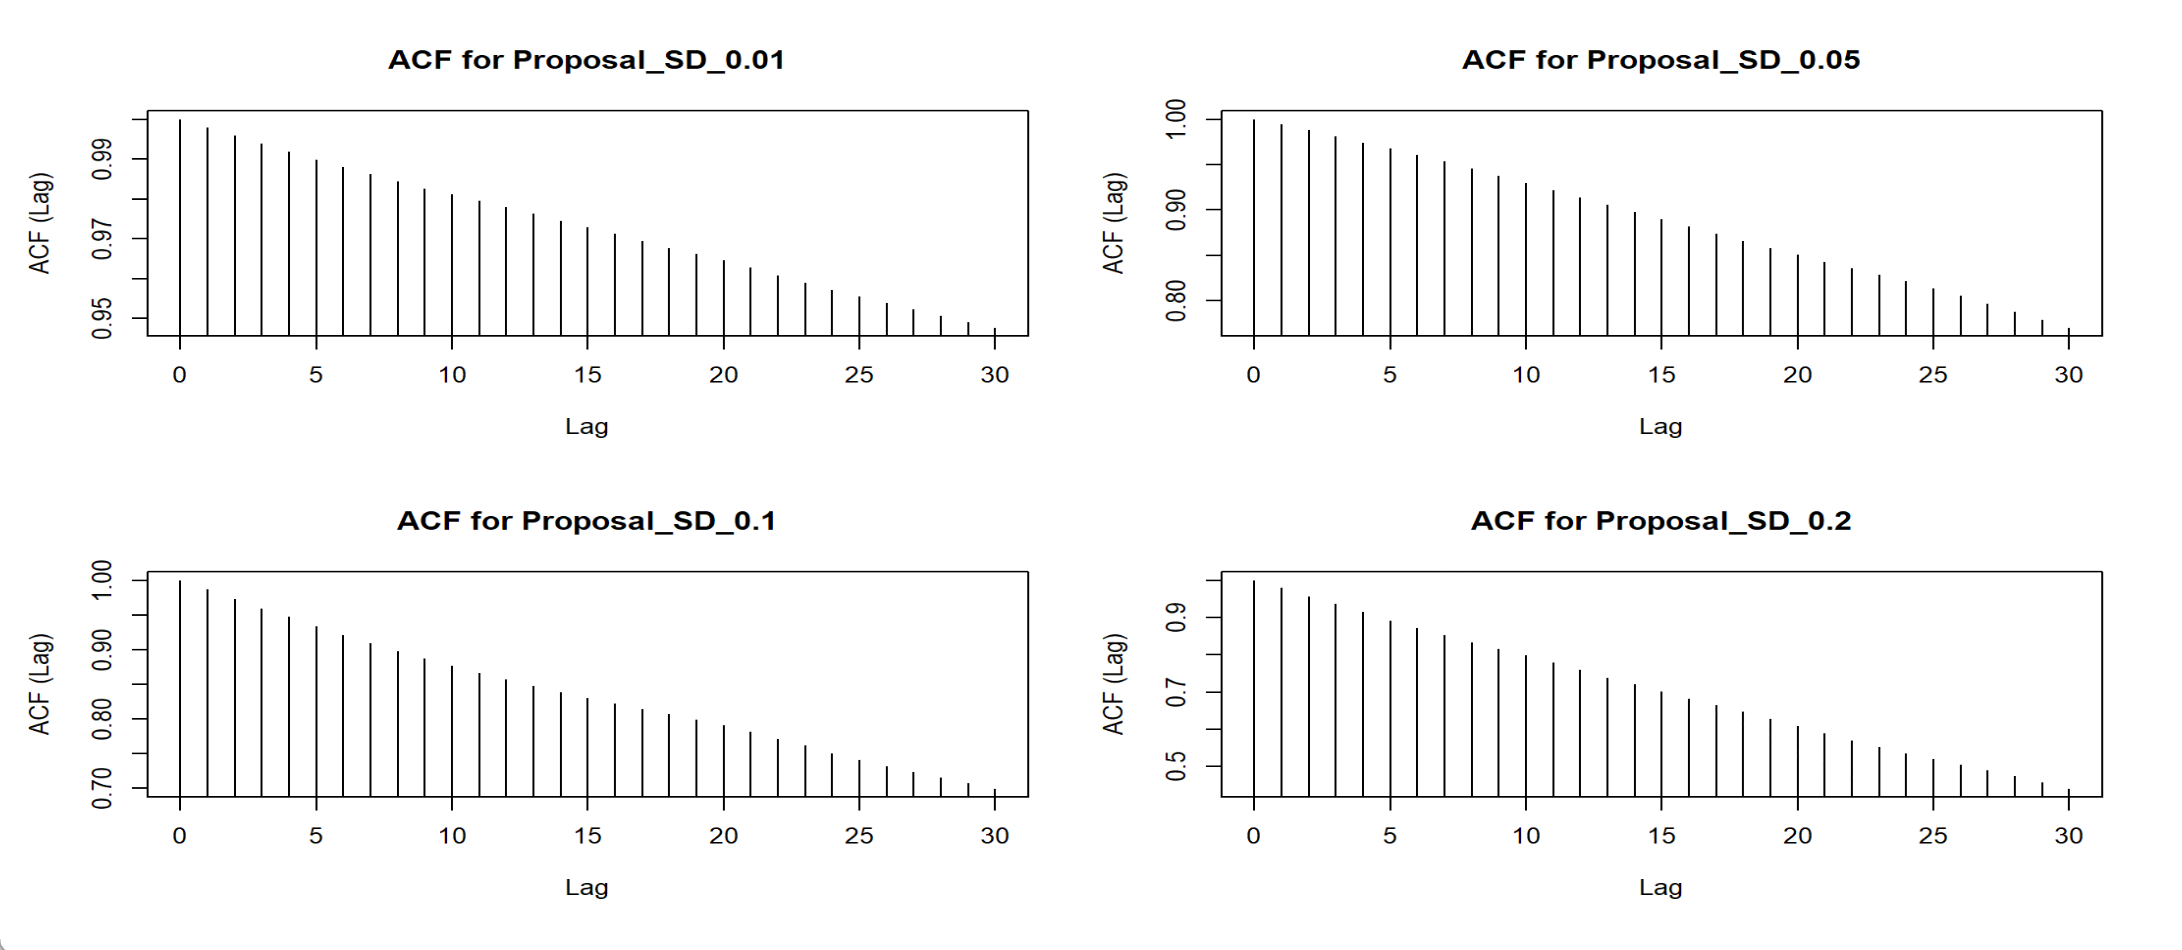
\includegraphics[width=1\linewidth]{01.png}
	\caption{不同提议分布方差下的自相关图} 
\end{figure}


\subsection{分析与归纳}
\subsubsection{提议分布方差对自相关系数的影响}
通过表格中的数据,我发现提议分布的方差增大时,相邻样本之间的自相关系数变小了;通过自相关图可以看出,随着提议分布方差的变大,自相关系数随着步数增大而下降的速率变大了,这说明了样本之间的关联性变小了。

\subsubsection{自相关性对参数估计准确性的影响}
随着自相关系数的减小,平均有效样本量也随之增加(但变化相对较小,这表明较高的自相关性并未显著降低有效样本量),这使得估计的均值更接近真实值,参数估计的准确性更高了。但是与之同时,估计的标准差也增大了。

\subsubsection{自相关性对置信区间宽度的影响}
随着自相关系数减小,置信区间的宽度明显地增大了,这是估计的方差增大导致的。

\section{总结}
本次实验主要通过Metropolis-Hastings算法进行MCMC采样,探索了不同提议分布方差对自相关性、参数估计准确性和置信区间宽度的影响。实验设置包括不同的提议分布方差(0.01、0.05、0.1和0.2),并通过50次独立实验进行模拟。

\subsection{研究结果总结}

\begin{itemize}
	\item **自相关性(ACF)**:随着提议分布方差的增大,自相关性逐渐降低。例如,当提议分布方差从0.01增加到0.2时,ACF值由接近1(非常高的自相关性)下降到较低的值,表明样本间的相关性减少。
	\item **参数估计准确性**:自相关性减弱一定程度上使估计的均值更接近真实值,但是也导致了较大的参数标准差,这反映了估计的不确定性增大。
	\item **置信区间宽度**:随着自相关性的减弱,置信区间宽度也显著增大,表明参数估计的精度下降,估计结果的不确定性增加。

\end{itemize}

这些结果表明,选择合适的提议分布方差对MCMC采样过程至关重要,它直接影响自相关性、参数估计的准确性和置信区间宽度。较大的方差能够减弱自相关性,从而使有效样本量增大,令估计地均值更接近目标分布的均值,但是会导致估计的方差和置信区间的宽度过大。

\subsection{未解决的问题与未来研究方向}

尽管本次实验提供了一些关于提议分布方差与自相关性、参数估计准确性之间的关系的初步结论,但仍存在一些未解决的问题和未来的研究方向:

\begin{itemize}
	\item **提议分布方差的选择**:当前的实验基于四种固定的提议分布方差进行测试。然而,如何根据具体问题自动选择最优的提议分布方差仍然是一个未解决的问题。未来可以研究如何通过自动调节提议分布的方差,以实现更高效的采样。
	\item **多维目标分布的研究**:目前的实验只考虑了简单的一维目标分布(正态分布)。对于更复杂的多维目标分布,Metropolis-Hastings算法的性能可能会有所不同。未来可以扩展实验,研究在高维空间下,提议分布方差对自相关性和估计准确性的影响,探索在多维目标分布中如何选择提议分布。
	\item **自适应Metropolis-Hastings算法**:传统的Metropolis-Hastings算法使用固定的提议分布方差,可能会导致效率低下或收敛缓慢。能否实现自适应Metropolis-Hastings算法,通过调整提议分布的方差来提高采样效率?未来的研究可以考虑引入自适应算法,使得提议分布在采样过程中根据样本的行为进行动态调整,从而提高MCMC采样的效率。
\end{itemize}

总的来说,虽然本次实验为提议分布方差对MCMC采样结果的影响提供了初步的定量分析,但在更复杂的采样问题中,如何优化提议分布的选择以及确保采样过程的收敛性和高效性,仍然是值得进一步探讨的研究方向。




\bibliographystyle{apalike}
\bibliography{ref.bib}


\clearpage

\appendix
\section{附录:代码}


\bigskip
\begin{lstlisting}
metropolis_hastings <- function(iter, initial_value, proposal_sd) {
	target_density <- function(x) {
		return(dnorm(x, mean = 0, sd = 1)) 
	}
	
	proposal_density <- function(x, current) {
		return(dnorm(x, mean = current, sd = proposal_sd)) 
	}
	
	samples <- numeric(iter)
	samples[1] <- initial_value
	
	for (i in 2:iter) {
		current <- samples[i - 1]
		proposed <- rnorm(1, mean = current, sd = proposal_sd)
		
		alpha <- min(1, target_density(proposed) / target_density(current))
		
		if (runif(1) < alpha) {
			samples[i] <- proposed
		} else {
			samples[i] <- current
		}
	}
	
	return(samples)
}

calculate_ESS <- function(samples) {
	acf_vals <- acf(samples, plot = FALSE)$acf[2] 
	ess <- length(samples) / (1 + 2 * sum(acf_vals))  
	return(ess)
}

monte_carlo_experiment <- function(iter = 1000, initial_value = 0, proposal_sds =
 c(0.01, 0.05, 0.1, 0.2), num_simulations = 50) {
	results <- list()
	
	for (sd in proposal_sds) {
		samples_list <- matrix(NA, nrow = num_simulations, ncol = iter)
		ess_list <- numeric(num_simulations) 
		
		for (i in 1:num_simulations) {
			samples_list[i, ] <- metropolis_hastings(iter, 
			initial_value, sd)
			ess_list[i] <- calculate_ESS(samples_list[i, ]) 
		}
		
		acf_vals <- apply(samples_list, 1, function(x) acf(x, 
		plot = FALSE)$acf[2]) 
		mean_acf <- mean(acf_vals)
		sd_acf <- sd(acf_vals)
		
		means <- apply(samples_list, 1, mean)
		sds <- apply(samples_list, 1, sd)
		ci_widths <- apply(samples_list, 1, function(x) {
			q <- quantile(x, c(0.025, 0.975))
			return(diff(q))
		})
		
		results[[paste("Proposal_SD", sd, sep = "_")]] <- list(
		samples = samples_list,
		mean_acf = mean_acf,
		sd_acf = sd_acf,
		mean = mean(means),
		sd = mean(sds),
		ci_width = mean(ci_widths),
		ess = mean(ess_list), 
		mean_se = sd(means) / sqrt(num_simulations),
		sd_se = sd(sds) / sqrt(num_simulations),
		ci_width_se = sd(ci_widths) / sqrt(num_simulations)
		)
	}
	
	return(results)
}

set.seed(123)
results <- monte_carlo_experiment(iter = 1000, initial_value = 0, proposal_sds = 
c(0.01, 0.05, 0.1, 0.2), num_simulations = 50)

for (sd in names(results)) {
	cat("\nResults for", sd, ":\n")
	cat("Mean ACF:", results[[sd]]$mean_acf, "\n")
	cat("SD of ACF:", results[[sd]]$sd_acf, "\n")
	cat("Estimated Mean:", results[[sd]]$mean, "\n")
	cat("Estimated SD:", results[[sd]]$sd, "\n")
	cat("Estimated CI Width:", results[[sd]]$ci_width, "\n")
	cat("Mean SE:", results[[sd]]$mean_se, "\n")
	cat("SD SE:", results[[sd]]$sd_se, "\n")
	cat("CI Width SE:", results[[sd]]$ci_width_se, "\n")
	cat("Average ESS:", results[[sd]]$ess, "\n")
}

par(mfrow = c(2, 2)) 
for (sd in names(results)) {
	samples <- results[[sd]]$samples[1, ]
	acf_vals <- acf(samples, plot = FALSE)
	plot(acf_vals$lag, acf_vals$acf, type = "h", main = paste("ACF for", sd), 
	xlab = "Lag", ylab = "ACF (Lag)")
}

\end{lstlisting}


\end{document}
